\documentclass{article}
\usepackage{tikz}
\usetikzlibrary{positioning}

\begin{document}

\begin{center}
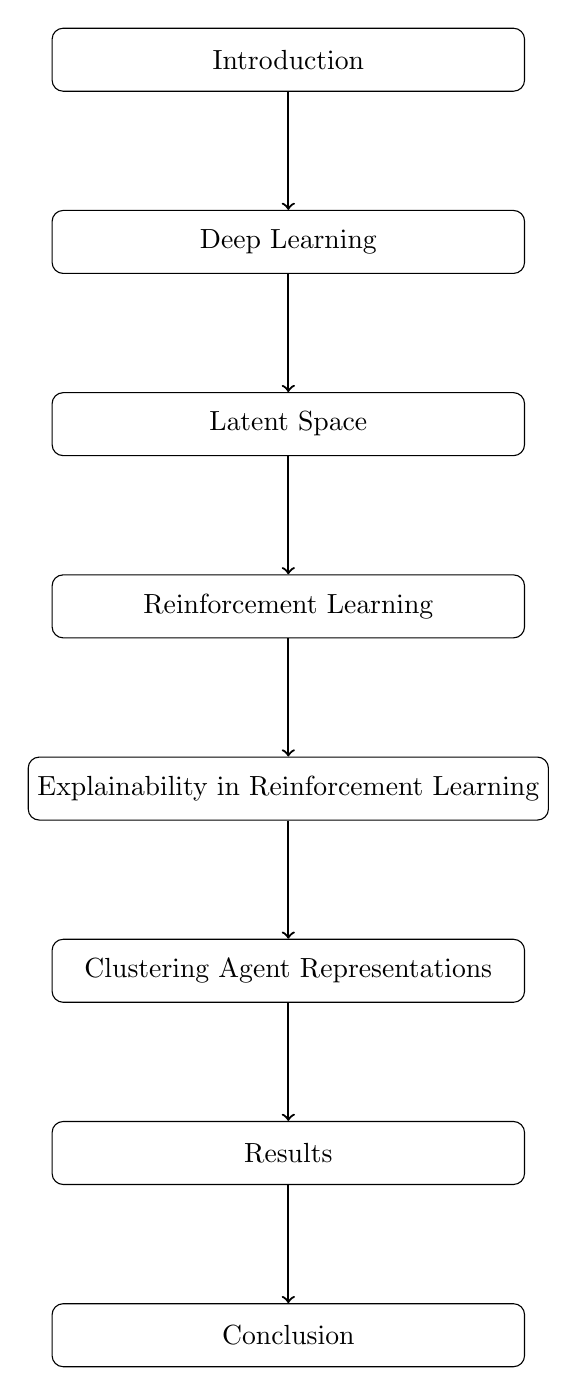
\begin{tikzpicture}[
    node distance=1.5cm,
    chapter/.style={
        rectangle,
        draw,
        rounded corners,
        minimum width=6cm,
        minimum height=0.8cm,
        align=center
    }
]

\node[chapter] (intro) {Introduction};
\node[chapter, below=of intro] (dl) {Deep Learning};
\node[chapter, below=of dl] (latent) {Latent Space};
\node[chapter, below=of latent] (rl) {Reinforcement Learning};
\node[chapter, below=of rl] (xrl) {Explainability in Reinforcement Learning};
\node[chapter, below=of xrl] (cluster) {Clustering Agent Representations};
\node[chapter, below=of cluster] (results) {Results};
\node[chapter, below=of results] (conclusion) {Conclusion};

\draw[->, thick] (intro) -- (dl);
\draw[->, thick] (dl) -- (latent);
\draw[->, thick] (latent) -- (rl);
\draw[->, thick] (rl) -- (xrl);
\draw[->, thick] (xrl) -- (cluster);
\draw[->, thick] (cluster) -- (results);
\draw[->, thick] (results) -- (conclusion);

\end{tikzpicture}
\end{center}

\end{document}